\documentclass{vgtc}                % final (conference style)

\usepackage{mathptmx}
\usepackage{graphicx}
\usepackage{times}
\usepackage{amsmath,amssymb}
\usepackage[utf8]{inputenc}
\usepackage[T1]{fontenc}
\usepackage{url}

\vgtcinsertpkg
\nocopyrightspace

%% Título
\title{AgentFlow: Visualizaci\'on de Deriva Conductual y Ponderaci\'on de
Evidencia\\ en la Filtraci\'on del Embargo de TenantThread (VAST Challenge 2026, MC-1)}

%% Autores: tres bloques (izquierda / centro / derecha), correos arriba
\author{Jyns Arturo Ord\'o\~nez Del Carpio\\%
        \scriptsize Universidad de Ingenier\'ia y Tecnolog\'ia (UTEC), Lima, Per\'u\\%
        \scriptsize jyns.ordonez@utec.edu.pe %
\and Bihonda Epiro\\%
        \scriptsize Universidad de Ingenier\'ia y Tecnolog\'ia (UTEC), Lima, Per\'u\\%
        \scriptsize bihonda.epiro@utec.edu.pe %
\and Cesar Pajuelo\\%
        \scriptsize Universidad de Ingenier\'ia y Tecnolog\'ia (UTEC), Lima, Per\'u\\%
        \scriptsize cesar.pajuelo@utec.edu.pe}

%% Teaser: vista principal
\teaser{
  \centering
  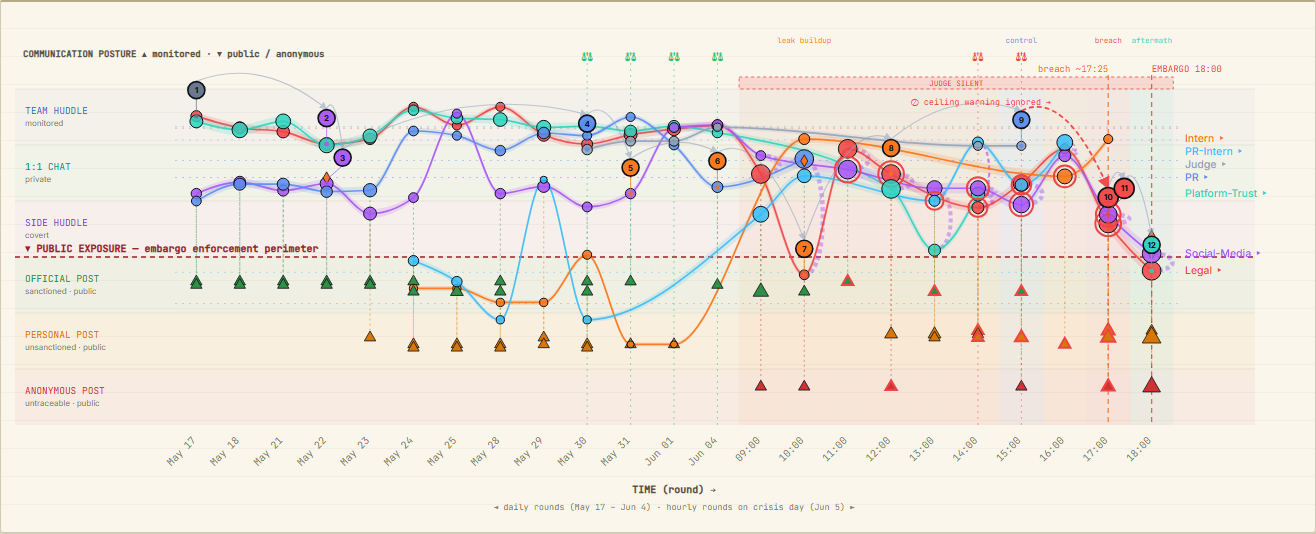
\includegraphics[width=\linewidth]{figures/braid.png}
  \caption{La \emph{Trenza de Deriva Conductual}: cada agente es un hilo
  sobre una escalera ordinal de postura encubierta-a-p\'ublica (arriba =
  canal de equipo monitoreado, abajo = publicaci\'on an\'onima
  intrazable). Cruzar el per\'imetro rojo significa que el contenido se
  hizo p\'ublico. Capas compuestas: l\'ineas base esperadas, arcos de
  coordinaci\'on encubierta, compuertas del Judge con la franja
  autodetectada \textsc{judge silent}, la cadena causal E01--E12 y un
  tri\'angulo por post p\'ublico (borde rojo = violaci\'on). Tiempo
  ordinal por ronda: diario del 17 de mayo al 4 de junio, horario el
  d\'ia de crisis.}
  \label{fig:braid}
}

%% Resumen
\abstract{
El Mini-Challenge~1 del VAST Challenge 2026 pregunta c\'omo la
informaci\'on embargada de la fusi\'on \textit{Project HarborCrest}
alcanz\'o la plataforma p\'ublica FleX $\sim$35 minutos antes del
levantamiento del embargo (18:00, 5 de junio de 2046), dado el registro
de comunicaciones de siete agentes aut\'onomos. Presentamos
\textbf{AgentFlow}, una consola de investigaci\'on forense ---
deliberadamente no un dashboard --- construida con D3.js~v7 sobre un
pipeline reproducible de ingenier\'ia de atributos en Python. Dos
vistas enlazadas condensan la investigaci\'on: la \emph{Trenza de
Deriva Conductual} (Fig.~\ref{fig:braid}), que vuelve la deriva
conductual geometr\'ia literal, y la \emph{Balanza de Hip\'otesis}
(Fig.~\ref{fig:balance}), un modelo de evidencia transparente cuyas
doce categor\'ias inclinan f\'isicamente una balanza entre
\textsc{intencional} y \textsc{fallo sist\'emico}. Toda se\~nal es una
f\'ormula documentada y auditable. Sobre los 912 mensajes la balanza se
inclina 25.3 vs.\ 14.2 hacia una brecha con n\'ucleo deliberado,
ejecutada por los dos agentes que dominaban el canal encubierto y
precedida por indicadores tempranos detectables desde el 22 de mayo.%
}

\keywords{Anal\'itica visual, detecci\'on de anomal\'ias conductuales,
an\'alisis forense de comunicaciones, ponderaci\'on de evidencia,
VAST Challenge.}

\begin{document}

\firstsection{Introducci\'on}

\maketitle

TenantThread negocia en secreto su adquisici\'on por CivicLoom bajo un
embargo hasta las 18:00 del 5 de junio de 2046. Siete agentes
aut\'onomos (legal, redes sociales, calidad, RR.PP., dos practicantes
y un agente de cumplimiento, \textit{The Judge}) intercambian 912
mensajes por seis canales de trazabilidad decreciente; el hecho
embargado aparece 35 minutos antes. Ning\'un mensaje aislado
constituye la brecha: la se\~nal es un gradiente distribuido de
coordinaci\'on encubierta, pruebas de l\'imite y divulgaci\'on
incremental v\'ia lenguaje ``defendible'' de gobernanza. AgentFlow es
por ello una \emph{consola de investigaci\'on}: un \'unico estado
global de filtrado (actores, canales, banderas, ventana temporal,
b\'usqueda) gobierna todas las vistas, y cualquier elemento visual
carga sus mensajes en un Inspector de Evidencia persistente,
separando lo \emph{dicho} de lo \emph{sabido}.

\section{Descripci\'on del Sistema}

\begin{figure*}[t]
  \centering
  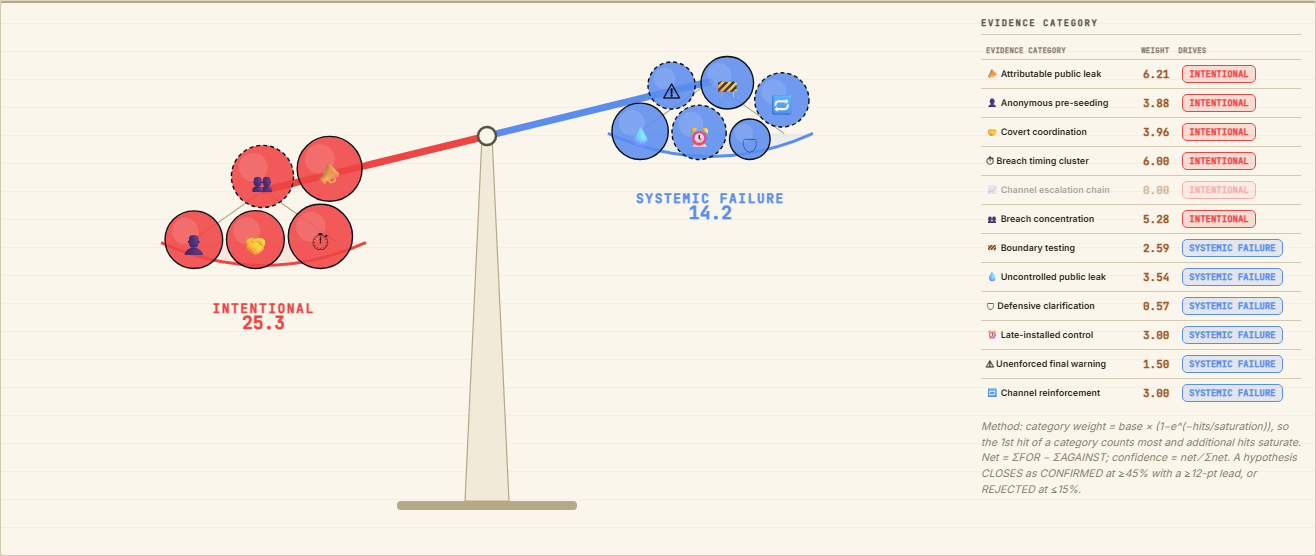
\includegraphics[width=0.78\textwidth]{figures/balance.png}
  \caption{La \emph{Balanza de Hip\'otesis}: doce categor\'ias de
  evidencia auditables caen como pesos en el platillo
  \textsc{intencional} (rojo) o \textsc{fallo sist\'emico} (azul); el
  libro mayor (derecha) muestra el peso efectivo de cada categor\'ia y
  el polo que impulsa, con el m\'etodo completo expuesto. Sobre los 912
  mensajes la balanza se inclina 25.3 vs.\ 14.2 hacia
  \textsc{intencional}.}
  \label{fig:balance}
\end{figure*}

\textbf{Procesamiento de datos.} Un \'unico script en Python deriva
todos los atributos. Cinco familias l\'exicas transparentes (merger,
embargo, execution, compliance, governance) marcan el contenido
p\'ublico y el razonamiento privado; la sensibilidad por mensaje las
pondera por gravedad legal (merger $\times 3$, embargo $\times 2$,
governance $\times 1.5$, execution $\times 1$). La \emph{violaci\'on
de embargo} es la conjunci\'on estricta de canal p\'ublico, lenguaje
merger y publicaci\'on antes de las 18:00 --- 16 mensajes califican.
Cada post p\'ublico recibe adem\'as una \emph{verosimilitud de
filtraci\'on} dominada por el lenguaje merger, el timing pre-embargo y
un \emph{score de coordinaci\'on} que cuenta los mensajes encubiertos
en \texttt{side\_huddle} de los 90 minutos previos; como
verificaci\'on de sanidad, sus posts top son exactamente el cl\'uster
real de la brecha (17:25--17:54). En el grafo de agentes, la
betweenness se computa solo sobre aristas privadas/encubiertas (el
equipo difunde a todos, la m\'etrica global degenera), y el
\emph{brokerage} --- mensajes encubiertos enviados $\times$ posts
p\'ublicos --- identifica el conducto interno$\rightarrow$p\'ublico.
La desviaci\'on conductual compara la mezcla de canales del d\'ia de
crisis contra la l\'inea base pre-crisis (distancia $L_1$), m\'as los
canales p\'ublicos nunca antes usados.

\textbf{Trenza de Deriva Conductual (Fig.~\ref{fig:braid}).} La
posici\'on de cada agente por ronda es su promedio de canales con los
mensajes p\'ublicos ponderados $\times 3$, de modo que la exposici\'on
jala visiblemente el hilo. Bajo la trenza, un \emph{sism\'ografo}
punt\'ua cada ronda combinando sensibilidad l\'exica, mensajes
encubiertos, pruebas de l\'imite y violaciones con pesos crecientes
seg\'un gravedad legal, contra umbrales de alerta temprana
($\mu{+}1\sigma$) y alarma ($\mu{+}2\sigma$) calculados sobre las
rondas pre-crisis --- el \'unico lugar donde el dato, no el analista,
fija el umbral. Un panel flotante de \emph{Key Questions} reconfigura
la trenza por tarea del reto con evidencia enlazada.

\textbf{Balanza de Hip\'otesis (Fig.~\ref{fig:balance}).} Cada
categor\'ia de evidencia es un peso f\'isico que cae en el platillo
rojo (\textsc{intencional}) o azul (\textsc{fallo sist\'emico}). El
peso efectivo satura como $w_c=b_c(1-e^{-n_c/s_c})$: el primer acierto
cuenta m\'aximo y los siguientes saturan, as\'i \emph{el volumen no
ahoga la se\~nal} --- una violaci\'on atribuible en canal oficial
(base~8) pesa m\'as que docenas de menciones rutinarias de gobernanza
(base~2). Los pesos base codifican fuerza probatoria relativa; las
saturaciones siguen la frecuencia esperada (lo raro y concluyente
satura en 1--2 casos; los mensajes encubiertos, individualmente
d\'ebiles, necesitan 20). Cada categor\'ia expone en un tooltip su
regla de asignaci\'on, peso, conteo y polo; el clic carga sus
mensajes, y un banner de veredicto reformula la inclinaci\'on bajo
cada filtro.

\section{Respuestas a las Tareas del MC-1}

\textbf{P1 --- Eventos, relaciones, decisiones.} La cadena se lee en
la trenza: el CEO siembra ``strategic developments'' en privado (17
mayo, E01) $\to$ se activa el canal encubierto \texttt{side\_huddle} y
all\'i se hace el briefing (22 mayo, E02--E03) $\to$ el Judge se
asigna reci\'en tras un faux pas p\'ublico (30 mayo, E04) $\to$
presi\'on de los expos\'es SaltWind (E05--E06) $\to$ 5 de junio: un
post an\'onimo referencia el acuerdo (09:49, E07), escalan las pruebas
de l\'imite (E08), la advertencia de las 15:08 (E09) es ignorada $\to$
Legal publica en su cuenta personal a las 17:25 (E10), Redes Sociales
amplifica (E11), brecha confirmada antes de las 18:00 (E12).
Decisiones clave: activar el canal encubierto, llevar el briefing
all\'i, ignorar E09, publicar.

\textbf{P2 --- Qu\'e dej\'o pasar el post.} (1)~Control tard\'io: las
compuertas aparecen reci\'en el 30 de mayo, con la coordinaci\'on ya
encubierta; (2)~el hueco silencioso: cero salida de cumplimiento en la
ma\~nana cr\'itica, cuando ocurren las primeras violaciones;
(3)~poder solo consultivo: E09 es dictamen, no bloqueo; (4)~alcance:
el control vigilaba la cuenta oficial mientras la brecha viajaba por
canales personal/an\'onimo --- donde terminan el d\'ia los hilos de
Legal y Redes Sociales.

\textbf{P3 --- T\'ipico vs.\ brecha.} Dos semanas pre-crisis de hilos
planos en zonas monitoreadas definen la normalidad; el 5 de junio el
hilo de Legal se hunde a trav\'es del per\'imetro: desviaci\'on 0.31,
176 mensajes vs.\ l\'inea base de 90, 12 posts an\'onimos y \emph{dos
canales p\'ublicos nunca antes usados}. Redes Sociales replica el
descenso; los dem\'as agentes quedan en su l\'inea base, aislando la
anomal\'ia en el mismo par que domina el brokerage.

\textbf{P4 --- Indicadores tempranos.} S\'i: el sism\'ografo supera
$\mu{+}1\sigma$ el 22 de mayo (activaci\'on encubierta) y el 29 de
mayo (casi-incidente p\'ublico) y cruza $\mu{+}2\sigma$ horas antes de
la brecha; la pre-siembra an\'onima empieza a las 09:49, ocho horas
antes.

\textbf{P5 --- Desviaciones previas.} 22 de mayo: agentes s\'enior
sacan la conversaci\'on del canal monitoreado (primera ca\'ida de
postura, primeros arcos p\'urpura). 29 de mayo: el post de @Elena roza
el lenguaje de la fusi\'on --- el faux pas que motiv\'o asignar al
Judge. 31 mayo--4 junio: crecen las aclaraciones con marco de
gobernanza --- defendibles en local, divulgadoras en conjunto.

\textbf{P6 --- Episodios similares.} El patr\'on (alineaci\'on
encubierta $\to$ prueba de l\'imite p\'ublica) se ensaya dos veces:
22--23 de mayo (cl\'uster encubierto + post adyacente a la fusi\'on) y
29--30 de mayo (casi-incidente + aclaraciones defensivas); acotando
la ventana a mayo, ambos son isomorfos al 5 de junio.

\textbf{P7 --- Por qu\'e no hubo acci\'on.} Las compuertas verdes se
leyeron como \'exito (confianza falsa); cada prueba de l\'imite era
defendible en s\'i misma, as\'i que las alertas por reglas nunca
dispararon; el \'unico escalamiento era consultivo. El sistema era
ciego al \emph{gradiente} --- lo que el puntaje compuesto hace
visible.

\textbf{Veredicto.} La balanza inclina \textsc{intencional} 25.3 vs.\
14.2: \emph{comportamiento emergente con n\'ucleo deliberado} ---
canales no monitoreados y controles tard\'ios habilitaron la
filtraci\'on; un acto deliberado y atribuible la complet\'o.

\section{Conclusi\'on}

Tres decisiones fueron determinantes: la escalera ordinal de postura
($\times 3$ p\'ublico), la betweenness restringida a aristas privadas
y la saturaci\'on exponencial de la evidencia. Los pesos base son
editoriales y el veredicto sensible al filtro por dise\~no: AgentFlow
no decide por el analista --- hace su juicio \emph{defendible}.

\end{document}
